\documentclass[12pt, fullpage, a4paper]{article}
\usepackage{graphicx, latexsym}
\usepackage{setspace}
\usepackage{apacite}
\usepackage{amssymb, amsmath, amsthm}
%\singlespacing
%\onehalfspacing
\doublespacing

\begin{document}
\title{Multiple Imputation of Squared Terms\protect}


\author{Gerko Vink$^{1,2,}$\thanks{Correspondence to: Gerko Vink, Department of Methodology and Statistics, PO Box 80140, 3508 TC Utrecht, the Netherlands. Tel: +31 (0)30 253 9140, Fax: +31 (0)30 253 5797, E-mail: \texttt{g.vink@uu.nl}}\;  and Stef van Buuren$^{1,3}$\protect\\
\newline\\
\small{\textsl{$^1$Department of Methodology and Statistics, Utrecht University, the Netherlands}\protect}\\
\small{\textsl{$^2$Division of Methodology and Quality, Statistic Netherlands, the Netherlands}\protect}\\
\small{\textsl{$^3$Department of Statistics, TNO Quality of Life, the Netherlands}\protect}\\
\newline\\
}
\date{}
\maketitle

\section*{Abstract}
We propose a new multiple imputation technique for imputing squares. Current methods yield either unbiased regression estimates, or preserve data relations. No method, however, seems to deliver both, which limits researchers in the implementation of regression analysis in the presence of missing data. Besides, current methods only work under a MCAR mechanism. Our method for imputing squares uses a polynomial combination. The proposed method yields both unbiased regression estimates, whilst at the same time preserving the quadratic relations in the data for both MAR and MCAR mechanisms. 

\section*{Keywords}
 Multiple Imputation, Polynomial combination, Quadratic relation, Regression estimate, Squared terms.

\section*{Bios}

Gerko Vink is a doctoral candidate at the Department of Methodology and Statistics, Utrecht University, the Netherlands. For his doctoral candidacy, he is also affiliated with the Division of Methodology and Quality, Statistic Netherlands, the Netherlands. His research interests are in the areas of incomplete data and optimization. 

Stef van Buuren is Professor at the Department of Methodology and Statistics, Utrecht University, Utrecht, the Netherlands, and is head of the Department of Statistics, TNO Quality of Life, Leiden, the Netherlands. He has published extensively in the fields of incomplete data, growth and development and item response theory.

\newpage
\section*{Introduction}
Multiple imputation (MI) is the method of choice for many incomplete data problems. MI incorporates the uncertainty about the missing data by creating $m>2$ imputed datasets.
Missing values are filled in under an \emph{imputation model}. The imputed data that results from the imputation model is then analyzed by the \emph{analysis model}. Separate analyses can be combined to get a single inference or set of estimates by making use of the combining rules derived by Rubin (1987)\nocite{RubinD1987}. 

The most critical part of MI is specification of the imputation model. It is widely accepted that the imputation model should embrace all relations of scientific interest. Usually, this is done by incorporating the variables of interest as main factors. However, things become less clear if the scientific model contains nonlinear terms. 

As an example, if we want to predict $Y$ from $X$ and its square $X^2$, then both $X$ and $X^2$ should be included in the imputation model. Leaving the term $X^2$ out of the imputation model will result in a downwards bias of the slopes when we perform a regression analysis on the imputed data. However, although it is generally agreed that all squares and interactions should be accounted for in MI, no consensus on how to do this has been reached. 

Von Hippel (2009) \nocite{vonhippe2009} reviewed several approaches to imputing squares. The  \emph{'transform, then impute'} method calculates the squares and interactions in the incomplete data for the cases that have missing no values, and then imputes the derived variable like any other variable. The \emph{'impute, then transform'} method imputes variables in their raw form, and then calculates the derived variable in the imputed data after imputation. These methods were compared to the \emph{passive imputation} method (Van Buuren, Boshuizen, and Knook 1999)\nocite{stef1999fcs}, implemented in the \texttt{mice} package in R (Van Buuren and Groothuis-Oudshoorn 2010)\nocite{vanbuuren2010}, and  the\nocite{royston2005} \emph{ice} command for Stata (Royston 2005). 

Von Hippel (2009) advises to use the transform-then-impute method, which delivers acceptable regression estimates but heavily distorts the relationship between $X$ and $X^2$.  Figure \ref{fig:sepvar} shows that for the transform-then impute method, imputations do not follow the relation in the population (observed) data. We agree with Von Hippel�s conclusion, but do not want to overlook that the transform-then-impute method yields combinations of imputed values that would never occur, had the data been observed. Such imputations are implausible and should be rejected on that ground. 

We must note that Von Hippel�s conclusions are based on a missing completely at random (MCAR) mechanism \cite{seaman2012multiple}, where the missingness does not depend on the data, which is a limitation in practice. An imputation method would be more powerful if it yields acceptable inference under the missing at random (MAR) mechanism, where the missingness may depend on the data, but must not depend on the missing data itself. 

Because existing methods for imputing squared terms are severely limited, we propose the \emph{polynomial combination} approach, which yields unbiased regression estimates, whilst at the same time preserving the consistency between the imputed values, for MAR and MCAR mechanisms. 

\section*{Method}
\subsection*{\textit{Formulation of the problem}}
The model of scientific interest is
\begin{equation}\label{Y}
Y = \alpha + X \beta_1 + X^2 \beta_2 + \epsilon
\end{equation}
with $\epsilon \sim N (0,\sigma^2)$. We assume that $Y$ is complete and that $X = (X_{obs}, X_{mis})$ and $X^2=(X^2_{obs}, X^2_{mis})$ are partially missing.
The problem is to find imputations for $X$ such that estimates of $\alpha$, $\beta_1$, $\beta_2$, and $\sigma^2$ are unbiased, whilst ensuring that the quadratic relation between $X$ and $X^2$ will also hold in the imputed data. 
\subsection*{\textit{Polynomial combination method}}
Define the polynomial combination $Z=(Z_{obs},Z_{mis})$ as the linear combination $Z=X\beta_1 + X^2\beta_2$. The idea is to impute the missing values in $Z$ instead of $X$ and $X^2$, followed by decomposing the imputed data $Z$ into components $X$ and $X^{2}$. Imputing $Z$ reduces the multivariate imputation problem to a univariate problem, which is easier to manage. 

Under the assumption that $P(Y,Z)$ is multivariate normal, we can impute the missing part of $Z$ as $Y\beta^\ast + \epsilon^\ast$. Here $\beta^\ast$ is a random draw from the posterior distribution of the linear regression of $Y$ on $Z$, and $\epsilon^\ast$ is a draw from the residual distribution $Z-Y\hat{\beta}$. In cases where the normal residual distribution is unrealistic, we can use predictive mean matching (pmm)(Little 1988)\nocite{little1988missing}.

The next step is to decompose $Z$ into $X$ and $X^2$. Under model \eqref{Y} this is straightforward. The imputed value $Z$ has two distinct real roots: 
\begin{align}
\label{xl} X_-  &=-\frac{1}{2\beta_2} \left ( \sqrt{4\beta_2Z + \beta_1^2} +\beta_1 \right )
\\ \label{xh} X_+   &= \frac{1}{2\beta_2} \left ( \sqrt{4\beta_2Z + \beta_1^2}-\beta_1\right  )
\end{align}
where the discriminant $\Delta = 4\beta_2Z+\beta_1^2$ must be greater than zero. The case $\Delta = 0$ occurs if and only if both $\beta_1$ and $\beta_2$ are exactly 0, resulting in just one distinct real root, namely $X_0=-\beta_1 / 2\beta_2$.  Since incorporating non-existent relationships in the analysis serves no further purpose, we assume that regression estimates are always unequal to 0.

Given this assumption, for any given $Z$, we can take either $X$=$X_-$ or $X$=$X_+$, and square it to obtain $X^2$. Either root is consistent with 
$Z=X\beta_1 + X^2\beta_2$, but choice among these two options requires care. Note that the minimum of the parabola is located at  $X_{min}=-\beta_1/2\beta_2$. If we choose $X_-$ for all $Z$,  then all imputed $X \leq X_{min}$ will correspond to points located on the left arm of the parabolic function. This is generally not as intended. A sampling mechanism to determine whether to choose from $X_-$ or $X_+$ for a given $Z$ is needed. 

The choice between the roots is made by random sampling, conditional on $Y$, $Z$ and their interaction $YZ$. Let $V=(V_{obs},V_{mis})$, where $V_{obs}$ is a binary random variable defined as 0 if $X_{obs} \leq X_{min}$ and 1 otherwise. We model the probability $P(V=1)$ by logistic regression as 
\begin{equation}\label{PV}
\textnormal{logit}P(V=1)=Y\beta_Y + Z\beta_Z + YZ\beta_{YZ}
\end{equation}
on the observed data. 
Assuming that the same model applies to the missing values in $X$ (i.e. that the missingness mechanism is ignorable),  we calculate the predicted probability $P(V=1)$. As a final step, a random draw from the binomial distribution is made, and the corresponding (negative or positive) root is selected as the imputation. This is repeated for each missing value.

\subsection*{\textit{Imputation algorithm}}
The procedure leads to the following algorithm for imputing squares:
\begin{enumerate}
\item Calculate $X_{obs}^2$ for the observed $X$
\item Use predictive mean matching to multiply impute $X_{mis}$ and $X_{mis}^2$ as if they were unrelated, resulting in imputations $X^*$ and $X^{*2}$.
\item Estimate the pooled estimates $\hat\beta_1$ and $\hat\beta_2$ by linear regression of $Y$ given $X = (X_{obs},X^*)$ 
and $X^2 = (X_{obs}^2,X^{*2})$
\item Calculate the polynomial combination $Z = X\hat\beta_1 + X^2\hat\beta_2$
\item Multiply impute $Z_{mis}$ by predictive mean matching, resulting in imputations $Z^*$
\item Calculate roots $X_-$ and $X_+$ given $\hat\beta_1$, $\hat\beta_2$ and $Z^*$ using equations (2) and (3)
\item Calculate the abscissa at the parabolic minimum/maximum $X_{min}=-\hat\beta_1/2\hat\beta_2$
\item Calculate $V_{obs}=0$ if $X_{obs}\leq X_{min}$, else $V_{obs}=1$ 
\item Impute $V_{mis}$ by logistic regression of $V$ given $Y$, $Z$ and $YZ$, resulting in imputations $V^*$
\item If $V^*=0$ then assign $X^*=X_-$, else set $X^*=X_+$
\item Calculate $X^{*2}$
\end{enumerate}
The imputations $Z^*$ will satisfy $Z^*=X^*\hat\beta_1+X^{*2}\hat\beta_2$.

\section*{Results}
To illustrate the polynomial combination method, we simulated and compared the performance of all methods discussed by Von Hippel (2009) against the polynomial combination method. Data were generated according to the model $Y = \alpha + X \beta_1 + X^2 \beta_2 + \epsilon$, where $X$ is randomly generated from a standard normal distribution. A larger sample size ($n=10000$) was chosen to demonstrate convergence. However, the method works well for smaller sample sizes. We fixed the population intercept $\alpha$ at 0 and the residual standard deviation $\sigma_{\epsilon}$ at 1. Deviations seem to be larger when the slope of both $X$ and $X^2$ are larger, hence the population slopes $\beta_1$ and $\beta_2$ were set to 1. 
Let $R$ be a response indicator with
\begin{align}
\label{R} R& = \left\{ \begin{array}{ll}1     &  \mbox{    if    } X \textnormal{ is observed}\\0 &  \mbox{    if    } X \textnormal{ is missing} \\ \end{array}\right..
\end{align}
and let $Z_{mis}$ denote the missing values in $Z$. Given these settings we created 50 percent joint missingness in $X$ and $X^2$ according to four missing-at-random (MAR) mechanisms that follow 
\begin{equation}
P(R=0|Z_{obs},Z_{mis}, Y)=P(R=0|Z_{obs}, Y)
\end{equation}
by using a random draw from a binomial distribution of the same length as $Y$ and of size 1 with missingness probability equal to the inverse logit
\begin{equation*}
P(R=0)=\frac{e^{a}}{(1+e^{a})}.
\end{equation*}
Setting $a=(-\bar{X}+X_{i})/SD_{X}$ gives 50 percent left-tailed MAR missingness. Right-tailed, centered and tailed MAR missingness can be created by setting $a=(\bar{X}-X_{i})/SD_{X}$,  $a=.75- [(\bar{X}-X_{i})/SD_{X}]$ and $a=-.75+[(\bar{X}-X_{i})/SD_{X}]$, respectively. Adding or substracting a constant moves the sigmoid curve, which results in different missingness proportions.

As an analysis we used linear regression to see whether the population values could be estimated after imputation. We repeated the analyses 100 times. 

The regression estimates after applying the polynomial combination imputation can be found in Table \ref{tab}. The estimated coefficients of the imputed $X$ and $X^2$, the coefficient of the intercept $\alpha$ and the residual standard deviation $\sigma_\epsilon$ are all close to their respective population values. Missingness mechanisms that involve the right tail show slightly larger deviations.
 
In contrast, Table \ref{tab} also displays the performance of the impute-then-transform method regression estimates under the same simulation conditions. The impute-then-transform method, yields biased regression estimates, even under MCAR.

Table \ref{tab} also shows the performance of the passive imputation method. Passive imputation performance is similar to the problematic performance of the impute-then-transform method, as both methods calculate $X^2$ afterwards. 

Finally, the transform-then-impute method yields unbiased regression estimates, but only for MCAR. Although some estimates are retrieved, performance is severely impaired under the MAR assumption (see Table \ref{tab}).

All in all, the polynomial combination method yields regression estimates that both unbiased and preserve the data relation between $X$ and $X^2$. The polynomial combination method also perfectly reproduces the population value relationship between $X$ and its square $X^2$ in the imputed data. See Figure \ref{fig:strawman} for a graphical representation of the population and imputed data relations between $X$ and $X^2$, as generated by the polynomial combination method. 

We also looked at the mean and covariance matrix as reproduced by the imputed data and compared it to the population values. The mean and covariance matrix of $(X,X^2,Y)$ are
\begin{equation}
 \mu=\begin{bmatrix} 
\;0\;\\
\;1\;\\
\;\beta_2\; 
\end{bmatrix} 
\quad \textnormal{and}\quad
\Sigma=\begin{bmatrix}
\;1&   &\;\\
\;0& 2&\;\\
\;\beta_1& 2\beta_2& 1+\beta_1^2+2\beta_2^2\; 
\end{bmatrix}
\end{equation}
A set of $k$ mean values can be pooled to a single residual mean value with 
\begin{equation}\label{deltamu}
\Delta_{\mu}=\frac{1}{k}\sum_{i=1}^k |\mu_i-m_i|
\end{equation}
where $m_i$ is the $i$th mean value for the imputed data. Likewise, a pooled residual covariance matrix can be created by
\begin{equation}\label{deltasigma}
\Delta_{\Sigma}=\frac{1}{k}\sum_{i=1}^k |\Sigma_i-S_i|
\end{equation}
where $S_i$ is the $i$th covariance matrix of the imputed data. Performing a small simulation of $n=100$ with various regression weights and combining the results with equations \eqref{deltamu} and \eqref{deltasigma}, yields the following pooled residual mean and covariance matrix.
\begin{equation}\label{covmatriximp}
 \Delta_{\mu}=\begin{bmatrix} 
\quad0.003\;\\
\;-0.004\;\\
\;-0.003\;
\end{bmatrix} 
\quad \textnormal{and}\quad
\Delta_{\Sigma}=\begin{bmatrix}
\;-0.004&   &\;\\
\;0& 0.007&\;\\
\;-0.004& 0& -0.012\; 
\end{bmatrix}
\end{equation}
The results in \eqref{covmatriximp} suggest that the mean and covariance matrix in the population data are accurately preserved in the imputed data. Given that only normal imputations that preserve the mean and covariance matrix from the population data can yield unbiased imputations, we can now confidently say that the polynomial combination method yields unbiased regression estimates and delivers transformed variable imputations that are consistent with each other. 

All computations in this study have been carried out in R and all imputations are generated with the \texttt{mice} package in R (Van Buuren and Groothuis-Oudshoorn, 2011) with $m=5$ multiple imputions. A \texttt{mice.impute.pc} method for use with \texttt{mice} is available on request from the first author. 

\section*{Conclusion}
The polynomial combination method as developed here provides unbiased estimates for problems where incomplete $X$ and $X^2$ are both in the complete data model. It merges imputation techniques and decomposition of the quadratic equation to obtain the same unbiased regression estimates as the basic transform-then-impute method, whilst preserving the relations between $X$ and $X^2$. Also, it performs well under both MCAR and MAR missingness mechanisms. Our advice is to use the polynomial combination method to impute transformed variables with squared relations. 

We note that the simulation conditions used are rather harsh. For example,  50 percent of $X$ is missing and some missingness mechanisms severely limit the amount of usable predictive information,  especially right-tailed MAR missingness. Also, note that imputations are based on just one covariate. In real life datasets, conditions for imputing the data are often much better. Yet, also for simpler incomplete data problems, the polynomial combination method yields the best possible inferences even though the difference with the results from other methods may be smaller. 

We limited our calculations and analyses to squares, which are essentially interactions between two identical variables. Interactions between different variables remain best imputed using the transform-then-impute method. The polynomial combination method can be generalized to more complex non-linear combinations. We expect that the proposed method also applies to problems in which the scientifically interesting model contains multiple versions or transformations of $X$, such as interactions between different variables, higher degree polynomial equations and perhaps even splines, which are essentially piecewise polynomials. Exploring such applications of the polynomial combination method is subject to future work.
\newpage
\bibliographystyle{apacite}
\bibliography{references}

\newpage
\begin{figure}[h]
  \centering
    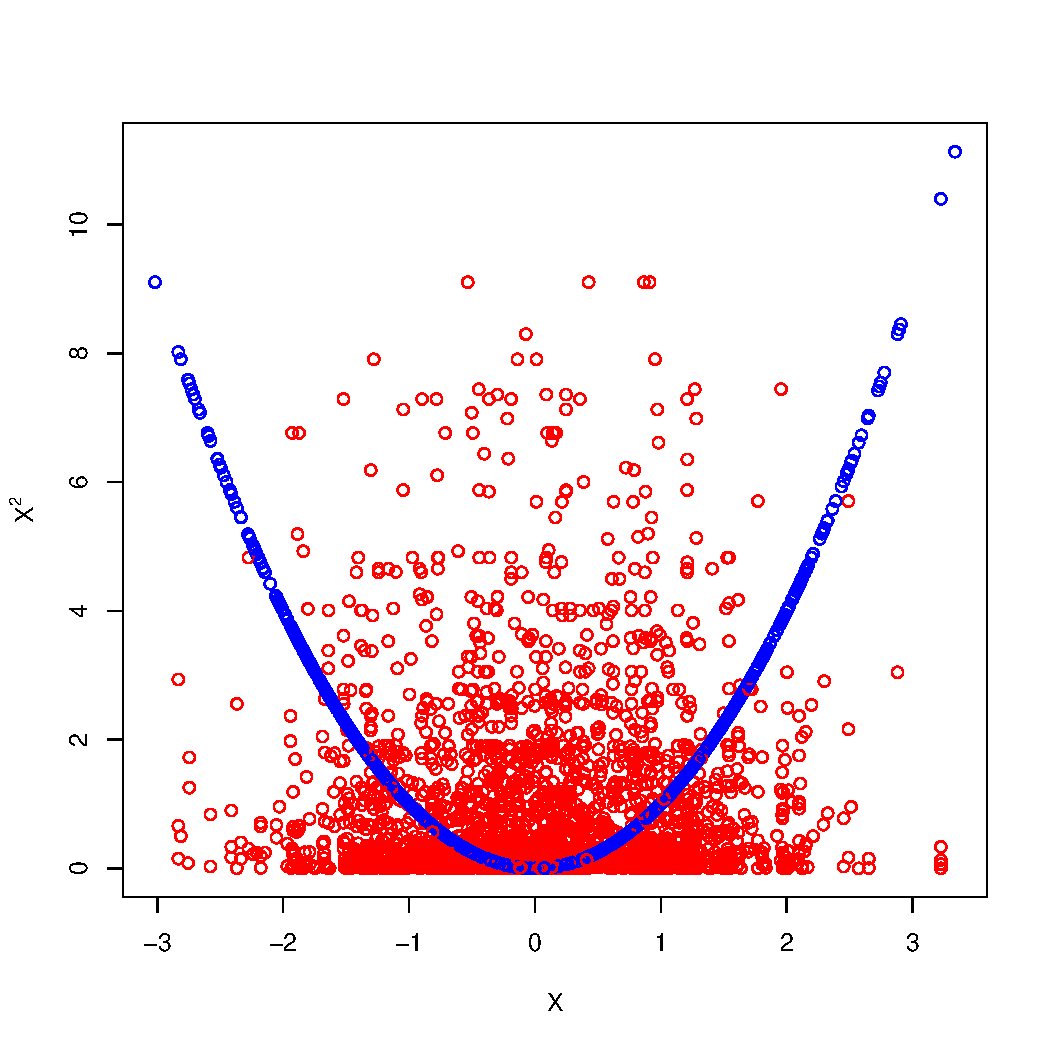
\includegraphics[scale=0.7]{sepvar.pdf}
  \caption{Transform-then-impute imputations. Observed (blue) and imputed values (red) for $X$ and $X^2$.}
  \label{fig:sepvar}
\end{figure}

%Grayscale version of Figure 1
%\newpage
%\begin{figure}[h]
%  \centering
%   \includegraphics[scale=0.7]{sepvar_graytone.pdf}
%  \caption{Transform-then-impute imputations. Observed (dark gray) and imputed values (light gray) for $X$ and $X^2$.}
%  \label{fig:sepvar}
% \end{figure}

\newpage
\begin{figure}[h]
  \centering
    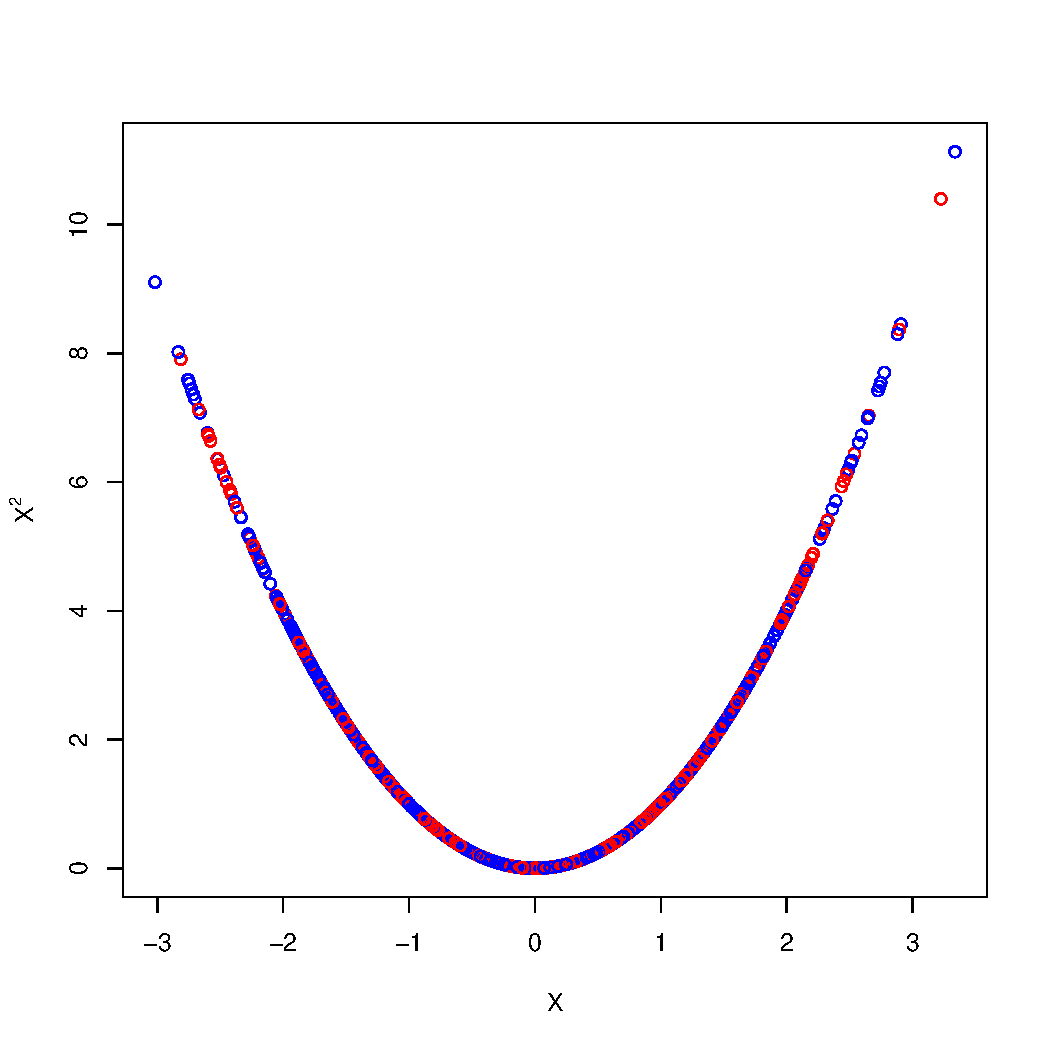
\includegraphics[scale=0.7]{polycomb.pdf}
  \caption{Polynomial combination imputation. Observed (blue) and imputed values (red) for $X$ and $X^2$.}
  \label{fig:strawman}
\end{figure}

%Grayscale version of Figure 2
%\newpage
%\begin{figure}[h]
% \centering
%    \includegraphics[scale=0.7]{polycomb_graytone.pdf}
%  \caption{Polynomial combination imputation. Observed (dark gray) and imputed values (light gray) for $X$ and $X^2$.}
%  \label{fig:strawman}
% \end{figure}


\begin{table}[h]
\begin{center}
\begin{tabular}{lcccccrl}
\hline
&\multicolumn{5}{c}{Missingness Mechanism} \\
\cline{2-6}
							&MCAR	&MARleft	&MARmid		&MARtail	& MARright\\
 \hline
\textit{Polynomial combination}	&&&&&\\
Intercept ($\alpha$)				&0		&-0.01	&-0.01	&-0.05	&-0.07\\
Slope of $X$ ($\beta_1$)			&1		&1		&1		&0.96	&0.96\\	
Slope of $X^2$ ($\beta_2$)		&1		&1		&1.01	&1.06	&1.09\\	
Residual SD ($\sigma_\epsilon$) 	&1		&1		&1		&1.03	&1.05\\	
$R^2$						&0.75	&0.75	&0.75	&0.73	&0.73\\\\
\textit{Impute, then transform}	&&&&&\\
Intercept ($\alpha$)				&0.39	&0.29	&0.26	&0.52	&0.56\\
Slope of $X$ ($\beta_1$)			&0.93	&0.94	&0.87	&1.01	&1.06\\
Slope of $X^2$ ($\beta_2$)		&0.61	&0.60	&0.67	&0.56	&0.66\\
Residual SD ($\sigma_\epsilon$) 	&1.48	&1.44	&1.41	&1.56	&1.62\\
$R^2$						&0.45	&0.48	&0.5		&0.39	&0.34\\\\
\textit{Passive imputation}	&&&&&\\
Intercept ($\alpha$)				&0.39	&0.29	&0.26	&0.52	&0.56\\
Slope of $X$ ($\beta_1$)			&0.93	&0.94	&0.87	&1.01	&1.05\\
Slope of $X^2$ ($\beta_2$)		&0.61	&0.60	&0.68	&0.56	&0.66\\
Residual SD ($\sigma_\epsilon$) 	&1.48	&1.45	&1.41	&1.57	&1.62\\
$R^2$						&0.45	&0.48	&0.50	&0.38	&0.34\\\\
\textit{Transform, then impute}	&&&&&\\
Intercept ($\alpha$)				&0		&0.19	&-0.13	&0.01	&-0.05\\
Slope of $X$ ($\beta_1$)			&1		&0.91	&0.97	&1.14	&1.32\\
Slope of $X^2$ ($\beta_2$)		&1		&0.91	&0.95	&1.14	&1.32\\
Residual SD ($\sigma_\epsilon$) 	&1		&0.95	&1		&1.06	&1.15\\
$R^2$						&0.75	&0.77	&0.75	&0.72	&0.67\\\hline
\end{tabular}
\caption{Average parameter estimates for different imputation methods under five different missingness mechanisms over 100 imputed datasets ($n=10000$) with 50\% missing data. The population parameters are $\alpha=0$, $\beta_1=1$, $\beta_2=1$,  $\sigma_\epsilon=1$ and $R^2=.75$}
\label{tab}
\end{center}
\end{table}




\end{document}